\documentclass[12pt,a4paper]{report}

\usepackage[utf8]{inputenc}
\usepackage[T1]{fontenc}
\usepackage[english]{babel}
\usepackage[top=1cm,bottom=2cm,left=1cm,right=1cm]{geometry}
%\usepackage{url}
%\usepackage{fancyhdr}
\usepackage{sectsty}
\usepackage{wrapfig}
\usepackage{titlesec}
\usepackage{setspace}
\usepackage{graphicx}
\usepackage{lmodern}
\usepackage{url}
\usepackage{amsmath}
\usepackage{amssymb}
\usepackage{mathrsfs}
\usepackage{fancyhdr}
\usepackage{gensymb}
\usepackage{enumerate}
\usepackage{caption}
\usepackage{hyperref} % Créer des liens et des signets 
\usepackage[cc]{titlepic}
\usepackage{listing}

\title{
\rule{15cm}{1pt} \\
\Large {\bfseries Machine Learning} \\
\Large {\bfseries Assignement 12 Conventional Neural Networks CNN}\\
\rule{15cm}{1pt}}
\author{Sami Sellami}

\titlepic{
\includegraphics[width=15cm]{Innopolis_image.png}} 
\date{\today}

\begin{document}
\pagenumbering{arabic}
\setcounter{page}{1}
\setcounter{secnumdepth}{1}
	
\fontfamily{ptm}\selectfont

\maketitle

\titlelabel{\thetitle)\quad}
\titlespacing{\chapter}{0cm}{0cm}{0cm}
\titlespacing{\section}{0.2cm}{0cm}{0cm}

THE SOURCE CODE IS ATTACHED TO THE PRESENT FILE 

\begin{enumerate}
\item Introduction:

Neural networks are notoriously difficult to configure and there are a lot of parameters that need to be set. On top of that, individual models can be very slow to train.
In this report we aim to use and compare two different methods (namely manual and Grid search) for tuning the parameters of a conventional neural network CNN on MNIST dataset.   

\item Implementation:

First we implement the manual search method, we test different values of each parameters while keeping the others constants and we repeat the operation for each parameters  	 

For our experiment we used the MNIST dataset which is a database of handwritten digits and has a training set of 60,000 examples, and a test set of 10,000 examples, the digits have been size-normalized and centered in a fixed-size image.

\begin{enumerate}
\item Tuning the batch size:

The batch size in iterative gradient descent is the number of patterns shown to the network before the weights are updated.
For our case,  we choose  different values of the batch size $B=[80, 100, 120, 140, 160,180]$, 
the following graph shows the accuracy obtained:

\begin{center}
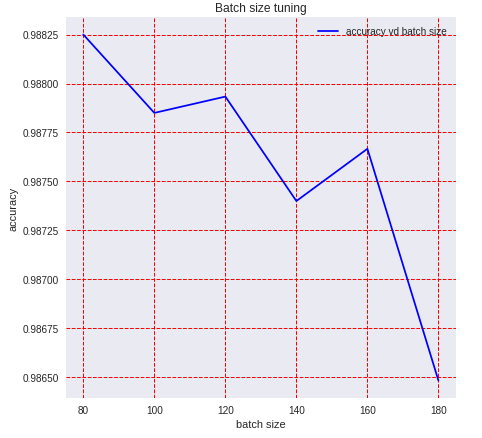
\includegraphics[width=7cm]{Capture1.png}
\captionof{figure}{Accuracy as a function of Batch size}
\end{center}

The result show that the batch size '80' gave the best accuracy 

\item Tuning the number of epochs:
The number of epochs is the number of times that the entire training dataset is shown to the network during training.
for our case we tried different values of epochs=
$[10, 20, 30, 40, 50]$ and with the batch size that we already found in the previous test batch size=80

\begin{center}
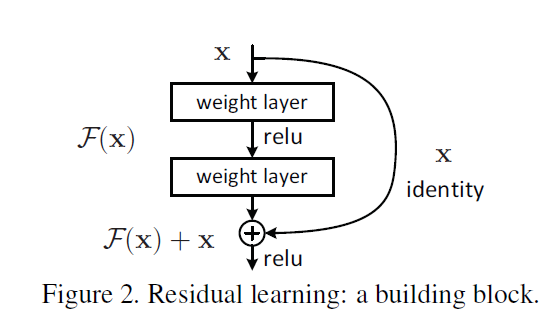
\includegraphics[width=7cm]{Capture2.png}
\captionof{figure}{Accuracy as a function of number of epochs}
\end{center}

We clearly see that the number of epochs '20' demonstrate the best accuracy

\item Tuning the Optimization method:
We use two different optimization method "Stochastic gradient descent (sgd)" and "Adam":  


\begin{center}
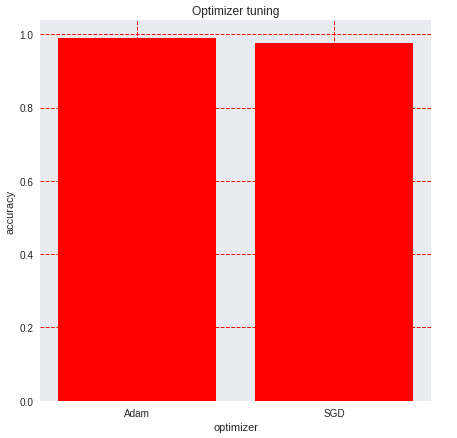
\includegraphics[width=6cm]{Capture3.png}
\captionof{figure}{Accuracy as a function of the optimization method}
\end{center}

We can see that the optimizer 'Adam' gave the best accuracy 

\item Tuning the Loss function:
We tried two candidates for the loss function of our CNN (categorical crossentropy and binary crossentropy) while keeping the other parameters constants and equal to the optimized ones found previously, the result is shown in the following graph

 
\begin{center}
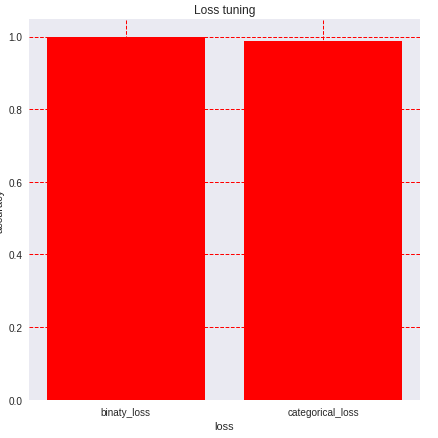
\includegraphics[width=6cm]{Capture5.png}
\captionof{figure}{Accuracy as a function of loss functions}
\end{center}

The candidate loss function binary crossentropy is the best one for our dataset because it demonstrated the highest accuracy 

\item Tuning the Number of hidden layers and units:
The number of neurons in a layer controls the representational capacity of the network, for our example we first tried  three different values of unit in one layer 64, 128 and 256 while keeping the other parameters constants and equal to the optimized ones found previously, then we changed the number of layers to 2 and 3,  the result is shown in the following graphs

\begin{center}
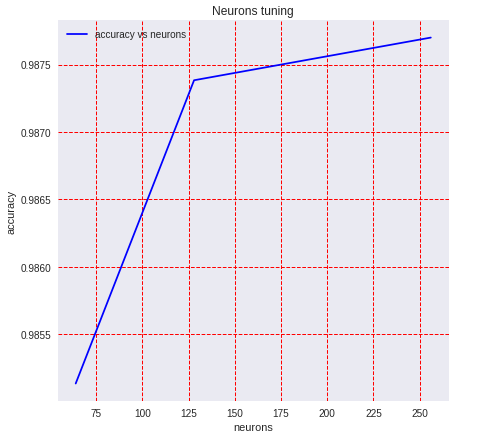
\includegraphics[width=6cm]{Capture4.png}
\captionof{figure}{Accuracy as a function of number of units in CNN with one layer}
\end{center}


\begin{center}
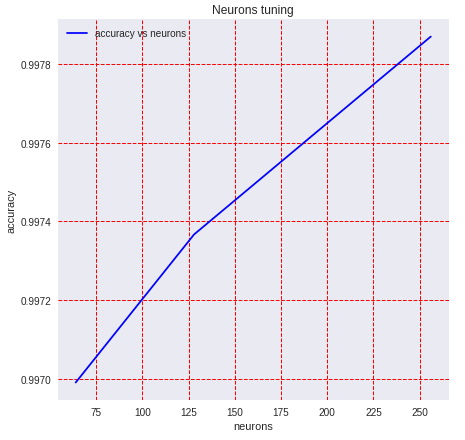
\includegraphics[width=6cm]{Capture6.png}
\captionof{figure}{Accuracy as a function of number of units in CNN with two layer}
\end{center}

\begin{center}
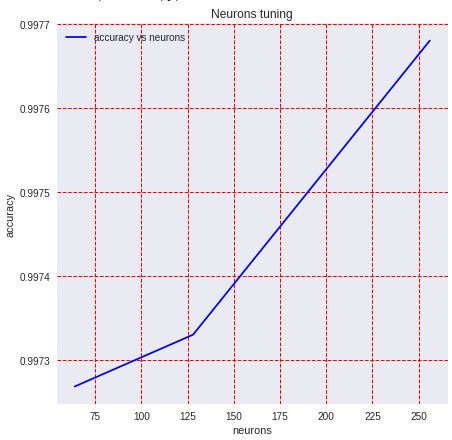
\includegraphics[width=6cm]{Capture7.png}
\captionof{figure}{Accuracy as a function of number of units in CNN with three layer}
\end{center}

We can see that the number of units in a hidden layers equal to '256' demonstrates the best accuracy in the three cases and, with three layers we obtain the highest accuray meaning the more layers we have the better


\item Tuning the activation function:
The activation function controls the non-linearity of individual neurons and when to fire.
We tried three different activation function namely 'relu' 'sigmoid' and 'tanh' while keeping the other parameters constants and equal to the optimized ones found previously, the result is shown in the following graph

 
\begin{center}
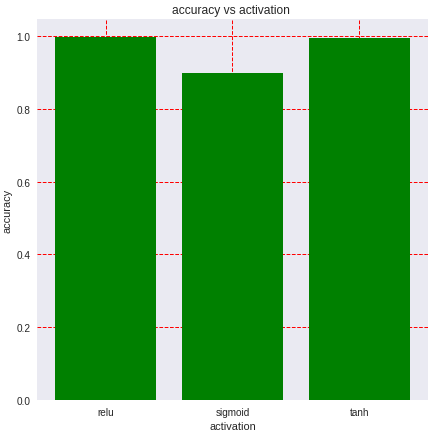
\includegraphics[width=6cm]{Capture8.png}
\captionof{figure}{Accuracy as a function of loss functions}
\end{center}

From the graph we conclude that the activation 'relu' is the best one for training our dataset
\\

With all these parameters set, ( 'activation': 'relu', 'batch size': 80, 'epochs': 20, 'loss': function binary crossentropy , 'neurons': 256, 'optimizer': 'Adam')
we obtained an accuracy of Best: 0.997298 which is better that the one at the beginning of our tests.
\\

\textbf{Discussion:}

This approach gave good results but it has some downwards, it doesn't give us information about which of the parameters should we train first and can theoretically give a completely different result for a different order of parameters tuning 
\\
\\

This is why we are going to use the second approach which consist on using the Grid search capability from the scikit-learn python machine learning library to tune the hyperparameters of Keras deep learning models.

When constructing this class we must provide a dictionary of hyperparameters to evaluate . This is a map of the model parameter name and an array of values to try.
By default, accuracy is the score that is optimized
\\

The GridSearchCV process will then construct and evaluate one model for each combination of parameters. Cross validation is used to evaluate each individual model.

However this method being very time and resources consuming, we split the hyper-parameters tuning into four different cases:

\begin{enumerate}
\item Fist case:

batch Size = [100,  140,  180]\\
epochs = [10, 20, 30]\\
optimizer = ['SGD']\\
neurons=[64, 128, 256]\\
loss = [binary crossentropy]\\
activation = ['relu']\\
\\
This is the  result of the implementation \\
Best: 0.992213 using {'activation': 'relu', 'batch size': 100, 'epochs': 30, 'loss': function binary crossentropy , 'neurons': 256, 'optimizer': 'SGD'}

\item Second case:

batch size = [100,  140,  180]\\
epochs = [10, 20, 30]\\
optimizer = ['adam']\\
neurons=[64, 128, 256]\\
loss = [categorical crossentropy]\\
activation = ['sigmoid']
\\

This is the  result of the implementation \\
Best: 0.912367 using {'activation': 'sigmoid', 'batch size': 140, 'epochs': 10, 'loss': categorical crossentropy, 'neurons': 64, 'optimizer': 'adam'}


\item Third case:

batch size = [100,  140,  180]\\
epochs = [10, 20, 30]\\
optimizer = ['SGD']\\
neurons=[64, 128, 256]\\
loss = [binary crossentropy]\\
activation = ['tanh']
\\

This is the  result of the implementation \\
Best: 0.989873 using {'activation': 'tanh', 'batch size': 100, 'epochs': 30, 'loss': binary crossentropy, 'neurons': 256, 'optimizer': 'SGD'}

We conclude that the best combination of hyperparameters that gave the best accuracy is the first one:
Best: 0.992213 using {'activation': 'relu', 'batch size': 100, 'epochs': 30, 'loss': function binary crossentropy , 'neurons': 256, 'optimizer': 'SGD'}

Of course this three cases are not reflecting all the possible situation but contrary to the manual approach, this is a very straightforward method 
\\

\item Fourth case:

batch size = [100,  140,  180]\\
epochs = [10, 20, 30]\\
optimizer = ['adam']\\
neurons=[64, 128, 256]\\
loss = [binary crossentropy]\\
activation = ['relu']\\

This is the  result of the implementation \\
Best: 0.998005 using {'activation': 'relu', 'batch size': 180, 'epochs': 30, 'loss': binary crossentropy , 'neurons': 256, 'optimizer': 'adam'}

\end{enumerate}

\textbf{Discussion:}
Comparing the cases we conclude that the fourth case is the best one for optimizing the network considering it give the highest accuracy (0.998005), one can also notice that this combination is approximately equal to the one for the manual search except for the batch size and the number of epochs 	  




\end{enumerate}

\item Conclusion:

In this report we presented two different approach for optimizing a Convolutional neural network using hyper-parameters tuning on MNIST dataset, the two methods shows good results in terms of the accuracy obtained with a higher accuracy for the grid search, however, each one has its pros and cons in term of efficiency, time computation and resources consumption, the manual method is direct and intuitive but it doesn't give information about which parameter should we train first, while GRID search test all possible combinations and give the best solution theoretically, but being very time and resources consuming it is practically hard to implement with large number of values and thus it is very restricting regarding the parameters tuning. 
     
\end{enumerate} 


\end{document}	
